%Linea Para poder completar automaticamente las citas con el Sublime
%No hace el documento, se puede borrar esta linea si no se usa el Sublime
%------------------------------------------------------------------------------
 \newcommand{\NoBiblioMeso}[1]{
 \ifthenelse{\equal{#1}{verdadero}}{}{\bibliography{Referencias/base_bibliografica}}
 \NoBiblioMeso{verdadero}}
 %-----------------------------------------------------------------------------

%Formato (Nombre de capitulo largo o corto), nombre del capitulo, resumen y estilo de la
%Portada del Capitulo
%------------------------------------------------------------------------------
 
 %Formato en si, titulo en dos renglones
 \FormatoCapituloDosLineas
 
 %Nombre y etiquete para referir
 \chapter{Métodos novedosos de síntesis de películas delgadas mesoporosas}
 \label{chap:Mesoporosos}

 %Para que no salga el numero de pagina en la portada del capitulo
 \thispagestyle{empty}
	
 %Resumen del Capitulo en Italica
 \noindent\textit{En este capitulos}
 %En capitulo explica como se sintetizaron y depositaron las películas mesoporosas sobre difrentes sustratos.  El objetivo fue probar la capacidad de adherencia, homogeneidad y espesor a la hora de depositar películas de óxido de silicio\index{silicio!oxido de}\index{silicio} mesoporoso en una variedad de sustratos. Establecer y estudiar las técnicas de caracterización para evaluar y analizar la porosidad, accesibilidad, conectividad\index{conectividad} con el objetivo último de evaluar la factibilidad de utilizarlos como sensores\index{sensor} electroquímico\index{electroquimico}s\index{electroquimico}.}
 
 
 %Indice de capitulo alineada al borde inferior de la pagina, nueva pagina
 \vfill
 \minitoc
 \newpage
 %-------------------------------------------------------------------------------

\section{Introducción}

	Existen una gran variedad precursor\index{precursor}es sensibles de condensar y determinar la estructura de películas delgadas mesoporosas de óxidos (PDM). Estas se pueden formar tanto de óxidos puros, como SiO$_2$, de Ti\index{titanio}O$_2$, Zr\index{circonio}O$_2$, o de óxidos de metales mixtos como Ti\index{titanio}Si, SiZr, por enumerar los precursor\index{precursor}es más utilizados. También existe una gran variedad de agentes moldeante para establecer el tamaño y la estructura espacial de los poros (F127, P123, Brij 58, CTAB, etc) \cite{angelome2011,schuth2013,Soler-Illia2006,Soler-Illia2002a}. Este trabajo se centró exclusivamente en síntesis de \pdm\space utilizando óxido de silicio\index{silicio!oxido de}\index{silicio} como precursor\index{precursor} para generar la estructura inorgánica. En la mayoría de los casos se utilizó puro y en algunos combinado con óxido de circonio\index{circonio} (ZrO$_2$). Para modelar el tamaño y estructura de los poros se utilizó el copolímero de bloque Pluronic F127\index{Pluronic F127} y bromuro de hexadeciltrimetilamonio\index{bromuro de hexadeciltrimetilamonio} (CTAB).Esta elección no fue arbitraria, sino que se hizo en base a premisas bien fundamentadas:
		
		\begin{enumerate}

		\item El SiO$_2$ es procesable por técnicas sol-gel\index{sol-gel} a través de diferentes precursor\index{precursor}es, es económico y fundamentalmente es el óxido mas utilizado en microelectrónica\index{microelectrónica}, aspecto fundamental en este trabajo para compatibilizar los procesos \textit{top-down}\index{top-down@\textit{top-down}} y \textit{bottom-up}\index{bottom-up@\textit{bottom-up}}.

		\item Ti\index{titanio}ene una química rica, bien conocida, forma enlaces covalentes con el carbono y es fácilmente funcionalizable pos-síntesis mediante el agregado de una gran variedad de grupos funcionales orgánicos o biológicos. Esta característica resultará fundamental para la selectividad de los sensores.

		\item No presenta absorción en el UV/Vis\index{UV}, esta característica es fundamental para poder hacer polimerizaciones dentro de los nanoporos sin tener interferencias por absorción de luz.

		\item Como agente moldeante\index{agente moldeante} se utilizó F127 ó CTAB de forma de obtener \pdm\space con tamaño de poros bien variados, de diámetros aproximados de \SI{10}{\nm} para el F127 y de \SI{2}{\nm} para el CTAB.

		\end{enumerate}
	
	Una vez elegidos los componentes esenciales que darán estructura a la película activa, se hizo foco en variar los sustratos. Ya que, al ser el objetivo final de la tesis sentar las bases para la fabricación de sensores\index{sensor} multiselectivos, se debían explorar las distintos soportes para las películas mesoporosas, de forma de poder abarcar un rango amplio de materiales para distintos usos.

	Se depositaron los soles\index{sol} sobre silicio\index{silicio} monocristalino, sobre vidrio\index{vidrio} y sobre películas delgadas de Au. En una primera etapa el objetivo fue el de estudiar el comportamiento de las \pdm\space sobre a diferentes sustratos. Para poder comparar los resultados con la bibliografía\cite{Soler-Illia2006,Brinker1990} se decidió, para esta etapa, depositar las películas por la ruta clásica de calcinación\index{calcinación}, explicada en la sección \ref{sec:cond_y_extr}, pág. \pageref{sec:cond_y_extr}. Impuestas estas condiciones de temperatura, se eligieron sustratos térmicamente estables:

		\begin{itemize}

			\item \textit{Portaobjetos de Vidrio}. Se utilizó para todo tipo de experimentos exploratorios, por ejemplo para pruebas de deposito, cortes o diseños, ya que es el mas económico que disponemos, de superficie\index{superficie} plana y con la misma composición que el sol, lo cual minimiza el estrés térmico sustrato-película.

			\item \textit{Silicio monocristalino, orientación cristalina [100]}. Las películas depositadas sobre silicio\index{silicio} se utilizaron para obtener resultados de espectroscopía de absorbancia IR, para hacer elipsoporisimetrías e imágenes MEB principalmente. El silicio\index{silicio} ofrece también un mayor contraste para visualizar las \pdm\space que el vidrio\index{vidrio} o el oro, por lo que se usó también para estimar la uniformidad de espesor por interferencia en toda la superficie\index{superficie} depositada.
		
			\item \textit{Películas delgadas de Au}. Estos sustratos fueron destinado para las pruebas electroquímica\index{electroquimico}s\index{electroquimico}, evaluar fenómenos de transporte, accesibilidad\index{accesibilidad} y propiedades de permeoselectividad. También se utilizó para imágenes de MEB.

			\end{itemize}
	
	En una segunda etapa, una vez dominada la química y física para obtener soles\index{sol} estables, películas homogéneas de espesor controlado y poder depositar sobre una amplia variedad de sustratos térmicamente estables, se dedicará el resto del capitulo a la discusión sobre métodos pos-depósito. 

	El desarrollo que se llevó a cabo sobre métodos de síntesis alternativos a la calcinación\index{calcinación} tienen varios própositos y surge de necesidades concretas. Por un lado, bajar la temperatura, permite compatibilizar los procesos \textit{bottom-up}\index{bottom-up@\textit{bottom-up}} (utilizados en la síntesis de las \pdm), y los procesos \textit{top-down}\index{top-down@\textit{top-down}} (necesarios para fabricar los sensores). Poro otro lado, permite incluir cada vez, materiales más diversos y, a su vez, poder tener mayores opciones a la hora de elegir de que forma fabricar los sensores\index{sensor} para aplicaciones dedicadas\cite{Doshi2000a,Wagner2013,Innocenzi2013,Soler-Illia2002a}.

	Para avanzar en esta dirección se explora una gama de procesos y condiciones químicas para sintetizar las películas delgadas mesoporosas reduciendo la temperatura por debajo de la temperatura de calcinación\index{calcinación}, típicamente de unos \SI{350}{\celsius}. Este proceso, que la mayoría de los autores emplean, tiene como ventaja, que promueve la condensación\index{condensación} del óxido y, a su vez, calcina el surfactante\index{surfactante} (materia orgánica) dando lugar a la formación de los poros.\cite{Zhang2015,Horiuchi2011,Clark2000,Zhang2005}

	La búsqueda de métodos de síntesis a bajas temperaturas permitiría fabricar los electrodos sobre Au\index{oro} metalúrgico o carbono (ver capitulo \ref{chap:Microfabricacion}, donde se desarrolla en profundidad estos aspectos) e incorporar sustratos poliméricos, como acrílico, resinas de poliéster, polibutileno de tereftalato (PBT), polietileno de tereftalato (PET), abriendo la posibilidad de utlizar una gama de materiales mucho mas amplia y abaratando costos.

	Veremos que mediante los procedimientos desarrollados es posible extender el uso de los sustratos considerablemente, abarcando virtualmente a cualquier superficie\index{superficie} de baja rugosidad\index{rugosidad} cuyo material sea estable por encima de los \SI{130}{\celsius}, incluyendo materiales poliméricos flexibles.
		
\section{Síntesis de películas delgadas mesoporosas}
		
		Para la síntesis de las películas mesoporosas se utilizaron modificaciones de los procesos conocidos como <<Autoensamblado inducido por evaporación>> desarrolladas por el grupo de Brinker.\cite{Brinker1999} En el capitulo \ref{chap:Introduccion}, pág. \pageref{sec:mesoporosos}, se hizo breve introducción sobre los aspectos teóricos de este proceso y en el capitulo \ref{chap:Materiales}, pág. \pageref{sec:sintesis_mesoporosos}, se detallan los aspectos experimentales para la obtención de las \pdm. Se recuerda la nomenclatura usada en el capítulo \ref{chap:Materiales}, \pdmF\space y \pdmC\space para películas delgadas mesoporosas de SiO$_2$ estructuradas con Pluronic F127\index{Pluronic F127} y CTAB respectivamente y \pdmZ\space para películas delgadas mesoporosas mixtas SiO$_2$/ZrO$_2$ estructuradas con F127.

		En los apartados que siguen a continuación se discuten los resultados obtenidos durante la fabricación de las \pdm\space por el método tradicional de calcinación\index{calcinación}. Se discuten detalladamente los aspectos para controlar la homogeneidad, adherencia, espesor y porosidad. Ésta será la base de conocimientos fundamentales para extrapolar y usar en el desarrollo de métodos de síntesis alternativos a la calcinación\index{calcinación} tratados en el resto del capítulo.

	\subsection{Control del espesor y homogeneidad}
		
		Las técnicas más utilizadas para el depósito\index{depósito} de películas por sol-gel\index{sol-gel} son \textit{dip-coating} y \textit{spin-coating}\index{spin@\textit{spin-coating}}. 
		Pensando en establecer las bases para la fabricación de sensores, se eligió trabajar exclusivamente por \textit{spin coating} con la intención de, en un futuro, escalar la síntesis, ya que esta técnica de síntesis es la que se utiliza en la industria de los semiconductores.\cite{Franssila2004,Jaeger2001} Primero se establecieron las rampas de aceleración y velocidad final del \textit{spinner}; los tiempos de estabilización en cámara de humedad; los tiempos de calentamiento y calcinación\index{calcinación}, de forma de obtener películas homogéneas, sin fisuras y del espesor deseado. Los detalles del proceso se encuentran en la sección \ref{sec:deposito_pdm} y \ref{sec:cond_y_extr}, pág. \pageref{sec:deposito_pdm}. 

		En la figura \ref{fig:fotos_films} se muestran fotografías de las \pdm\space obtenidas para los surfactante\index{surfactante} utilizados y los distintos sustratos. 

			\begin{figure}[th]
	 	   	    \begin{subfigure}[t]{0.325\textwidth}
		        	\includegraphics[width=0.95\textwidth]{Imagenes/CTAB-Si.jpg}
		       		\caption{\pdmC\space sobre una oblea\index{oblea} de silicio.}
		         	\label{fig:F127_vidrio}
		     		\end{subfigure}
	     		\begin{subfigure}[t]{0.325\textwidth}
		        	\includegraphics[width=0.95\textwidth]{Imagenes/CTAB-Au.jpg}
		       		\caption{\pdmC\space sobre un electrodo de Cr\index{cromo}\textbar Au.}
		         	\label{fig:F127_silicio}
		     		\end{subfigure}
	     		\begin{subfigure}[t]{0.325\textwidth}
		        	\includegraphics[width=0.95\textwidth]{Imagenes/CTAB-electrodo.jpg}
		       		\caption{\pdmC\space sobre un arreglo de electrodos (diseño 1).}
		         	\label{fig:F127_Au}
		     		\end{subfigure}
	 	   	    \begin{subfigure}[t]{0.325\textwidth}
		        	\includegraphics[width=0.95\textwidth]{Imagenes/F127-Si.jpg}
		       		\caption{\pdmF\space sobre una oblea\index{oblea} de silicio.}
		         	\label{fig:CTAB_vidrio}
		     		\end{subfigure}
	     		\begin{subfigure}[t]{0.325\textwidth}
		        	\includegraphics[width=0.95\textwidth]{Imagenes/F127-Au.jpg}
		       		\caption{\pdmF\space sobre un electrodo de Cr\index{cromo}\textbar Au.}
		         	\label{fig:CTAB_silicio}
		     		\end{subfigure}
	     		\begin{subfigure}[t]{0.325\textwidth}
		        	\includegraphics[width=0.95\textwidth]{Imagenes/F127-electrodo.jpg}
		       		\caption{\pdmF\space sobre un arreglo de electrodos (diseño 2).}
		         	\label{fig:CTAB_Au}
		     		\end{subfigure}
	     		\caption[Películas mesoporosas sobre distintos soportes.]{Fotografías de las \pdm\space obtenidas por \textit{spin-coating }sobre distintos soportes para los dos surfactante\index{surfactante}s utilizados: F127 y CTAB.}
	     		\label{fig:fotos_films}\index{spin@\textit{spin-coating}}
	     	   	\end{figure}

		Allí se pueden destacar dos características de las \pdm, la continuidad ya que no se ven ni grietas ni fisuras y la homogeneidad en el color, que es es indicador de un espesor constante a lo largo de la superficie\index{superficie} (salvo en los bordes debido, precisamente, a los efectos de borde generados por el giro del \textit{spinner})\cite{Franssila2004,Jaeger2001}.

		La ausencia de discontinuidades microscopicas (grietas o fisuras) se pudo corroborar con imágenes MEB, donde se ve que el depósito\index{depósito} es homogéneo en la superficie\index{superficie} (ver figura \ref{fig:sem_homogeneidad}). En dichas imágenes también se observan detalles del arreglo poroso, y, en el caso del F127 se ve que el arreglo poroso esta homogéneamente distribuido también a lo largo del eje transversal a la superficie\index{superficie}, como se muestra en la ampliación de la figura \ref{fig:sem_homogeneidad2}.

			\begin{figure}[th]
		 	   	    \begin{subfigure}[t]{0.49\textwidth}
			        	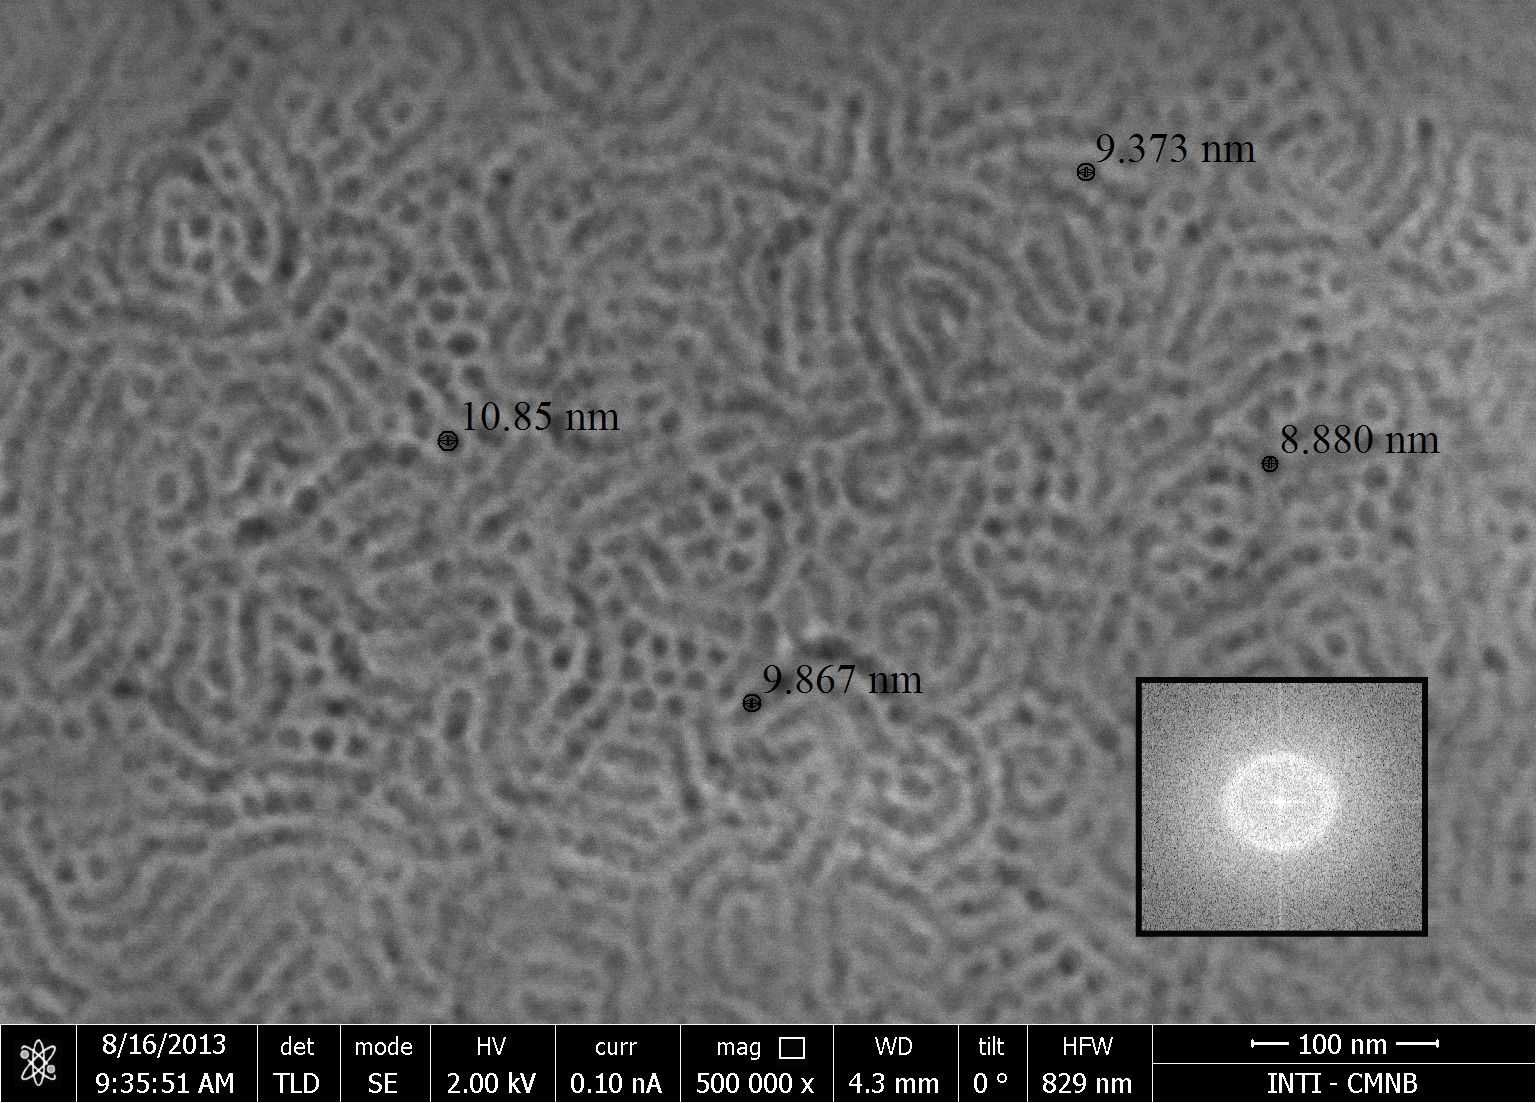
\includegraphics[width=\textwidth]{Imagenes/Superficie-F127-medidas.jpg}
			       		\caption{Microscopía electrónica donde se observa la superficie\index{superficie} de una \pdmF\space con poros de \SI{10}{nm} de diámetro en promedio.}
			       		\label{fig:sem_homogeneidad1}
			       		\end{subfigure}
					\begin{subfigure}[t]{0.49\textwidth}
			 	   	    \includegraphics[width=\textwidth]{Imagenes/Perfil-F127-modificado2.jpg}
			       		\caption{Corte transversal por FIB\index{FIB} de una \pdmF\space desde se puede medir el espesor y ver los nanoporos a lo largo del eje transversal a la película.}
			       		\label{fig:sem_homogeneidad2}
			       		\end{subfigure}
			       	\begin{subfigure}[t]{0.49\textwidth}
			        	\includegraphics[width=\textwidth]{Imagenes/Superficie-CTAB-medidas.jpg}
			       		\caption{Microscopía electrónica donde se observa la superficie\index{superficie} de una \pdmC\space con poros de \SI{3}{nm} de diámetro en promedio.}
			       		\label{fig:sem_homogeneidad3}
			       		\end{subfigure}
					\begin{subfigure}[t]{0.49\textwidth}
			 	   	    \includegraphics[width=\textwidth]{Imagenes/Perfil-CTAB.jpg}
			       		\caption{Corte transversal por FIB\index{FIB} de una \pdmC\space desde se puede medir el espesor de la película. Los nanoporos no se llegan a observar por ser de tamaño muy pequeño para la técnica utilizada.}
			       		\label{fig:sem_homogeneidad4}
			       		\end{subfigure}	
					 \caption[MEB \pdmC\space y \pdmF.]{Microscopia para sistemas de sílice porosos con CTAB y F127 calcinados sobre silicio\index{silicio} con electrodos de Cr\index{cromo}\textbar Au\index{oro} (a y c). Secciones transversales donde se puede apreciar la homogeneidad en el espesor de las películas (b y d).}
					 \label{fig:sem_homogeneidad}	
				     \vspace*{0.2cm}
				     \end{figure}

		El control del espesor se logra variando las condiciones de aceleración y velocidad final del \textit{spin-coater}, por lo tanto, para cada condición, se obtiene un espesor diferente. Las rampas que se han utilizado se muestran en la figura \ref{fig:spin}. El espesor de las \pdm\space se midió indistintamente por elipsoporosimetría\index{elipsoporosimetría ambiental} ambiental (EPA) o por microscopia\index{microscopía} (FIB/SEM), se puede consultar los detalles de las técnicas en las correspondientes secciones del capítulo \ref{chap:Materiales}. En el gráfico de la figura \ref{fig:esp} se muestra la curva de espesores que corresponde a un sistema nanoporoso de SiO$_2$ utilizando F127 como surfactante\index{surfactante}. 

		Según algunos autores, el tratamiento teórico para el deposito de películas poliméricas por \textit{spin-coating}\index{spin@\textit{spin-coating}} revela una dependencia del espesor con la velocidad según \cite{Norrman2005,Meyerhofer1978,Bornside1989,Lora1990}:
			\begin{equation}
			  t = k_1 \omega^{\alpha}
			  \label{eq:spin_meso}
			  \end{equation}		
		donde $k_1$ y $\alpha$ son constantes empíricas que dependen de la concentración del monómero, del solvente, del sustrato, de la interacción sol/sustrato y  de las propiedades reológicas del sol. Tal como se mostró en la ecuación \ref{eq:spin_meso}, y siguiendo los reportes de la literatura, el valor de $\alpha$ parece mantenerse contante y en las cercanías de $\alpha=-0.5$ para una gran cantidad de polímeros. Ajustando los valores del gráfico \ref{fig:esp} se obtienen los valores de $k_1=6413$ y  $\alpha=-0.442$, los cuales siguen la tendencia esperada; disminución del espesor con el aumento de la velocidad angular\index{velocidad!angular} y decaimiento exponencial con $\alpha \approx -0.5$. \marginpar{Quizás acá debe hacer la curva de calibración de espesores para el CTAB, que no la tengo.}
			\begin{figure}[!ht]
						\begin{center}
						\includegraphics[width=0.70\textwidth]{Graficos/Esp_F127.pdf}
						\caption[Espesor en función de la velocidad de rotación\index{velocidad!de rotación}.]{Espesor en función de la velocidad de rotación\index{velocidad!de rotación} para sistemas \pdmF con velocidades angulares comprendidas en 1000 y \SI{4000}{\minute^{-1}.}}
						\label{fig:esp}
						\end{center}
						\end{figure}

	\subsection{Discusión sobre la adherencia\index{adherencia} de las \pdm}	

		 En numerosos trabajos se ha demostrado la producción de películas delgadas mesoporososas de sílice (tanto con F127 como con CTAB) sobre sustratos de vidrio\index{vidrio} o silicio. Sin embargo, en ninguno se menciona la existencia de problemas de adherencia\index{adherencia} al sustrato\index{sustrato} \cite{Angelome2008,Fuertes2010,Violi2015}. Es más, se conoce que luego de ,tratamientos térmicos para condensar y calcinar el surfactante\index{surfactante}, las películas sufren una contracción uniaxial a lo largo del eje normal a la superficie\index{superficie} del sustrato\index{sustrato} debido a la fuerte adherencia\index{adherencia} al sustrato.\cite{Grosso2004,Soler-Illia2012,Chougnet2005} Se sabe desde hace décadas, que los metales nobles no tienen una buena adherencia\index{adherencia} sobre sustratos no-metálicos\cite{Kern1990,Hieber1976}, con lo cual es de esperar que también se experimenten problemas de adherencia\index{adherencia} al querer depositar un sol\index{sol} sobre una película delgada \index{película!delgada}de Au. 

		\subsubsection{Adherencia de \pdm\space sobre electrodos de Au\index{electrodo!de Au}}

			En el caso en los cuales se depositó \pdm\space estructuradas con Pluronic F127\index{Pluronic F127} sobre películas de Au, se observó, en algunos casos, falta de adherencia. Por ejemplo, en el gráfico \ref{fig:adherencia_F127}, se observa se <<despega>> la \pdm\space durante la adsorción\index{adsorción} de \aminorutenio. La forma del voltagrama (tanto los cambios en la intensidad como los corrimientos en el potencial) se discuten en profundidad en el capitulo \ref{chap:Electroquimica}. Por ahora nos basta con decir que se trata de un cambio repentino de un ciclo de medición al siguiente, pasando de la típica respuesta de una \pdm, a la respuesta habitual de un electrodo desnudo de Au. Esta respuesta sugiere que la película no sufrió una disolución lenta y paulatina, sino que se desprendió del sustrato, total o parcialmente, en algún momento de la medición.
			
				\begin{figure}[th]
				 	   	    \begin{center} 
				        	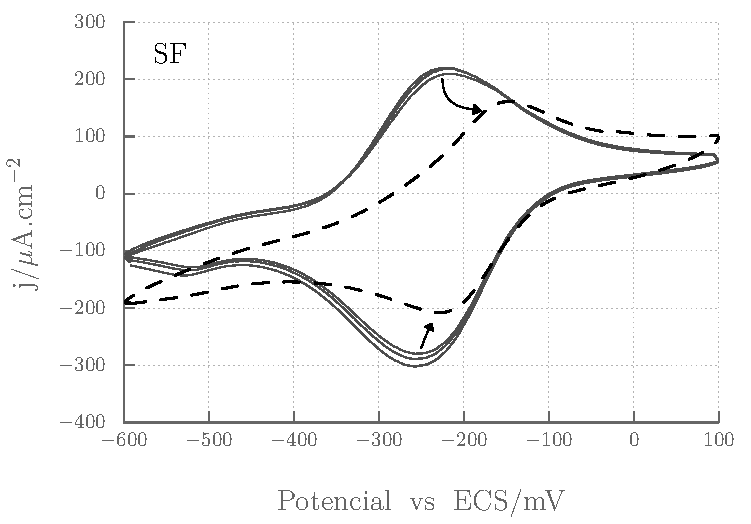
\includegraphics[width=0.70\textwidth]{Graficos/Adherencia_F127.pdf}
				       		\caption[Adherencia de \pdmF \space sobre una película delgada \index{película!delgada}de Au.]{Serie de voltametrías cíclicas consecutivas donde se evidencia la falta de adherencia\index{adherencia} de \pdmF \space sobre electrodo de Au\index{electrodo!de Au}. Las flechas negras indican un cambio repentino de comportamiento. Las VC fueron tomadas a \SI{50}{\milli\volt.\second^{-1}} usando de referencia ESC y con de \ru\space \SI{1}{\milli\Molar}.}
				         	\label{fig:adherencia_F127}
				     		\end{center}
				     		\end{figure}

			En los casos en los cuales se utilizó CTAB como molde para los poros, el comportamiento es algo diferente. Se ven problemas de adherencia\index{adherencia} en la mayoría de los tratamientos alternativos, así como en la calcinación\index{calcinación}. Presentan grietas y fisuras, macro y microscopicas y se observan desprendimientos antes de someter los sensores\index{sensor} a cualquier medición, es decir, apenas terminada la síntesis. Solo se rescataron algunos pocos casos exitosos de formación de \pdmC\space por calcinación\index{calcinación} utilizando como soporte electrodos de Au\index{electrodo!de Au}. Éstos sirvieron para hacer experimentos de EQ conceptuales sobre transporte\index{transporte} en poros (consultar capitulo \ref{chap:Electroquimica}), pero en la generalidad de los casos se observa desprendimiento de la película tal como muestran las imágenes de la figura \ref{fig:CTAB_adherencia}.
	     
				\begin{figure}[th]
		 	   	    \begin{subfigure}[t]{0.49\textwidth}
			        	\includegraphics[width=\textwidth]{Imagenes/Au_FCCTAB_adherencia1.jpg}
			       		\end{subfigure}
					\begin{subfigure}[t]{0.49\textwidth}
			 	   	    \includegraphics[width=\textwidth]{Imagenes/Au_FCCTAB_adherencia2.jpg}
			       		\end{subfigure}
					 \caption[Adherencia de CTAB sobre electrodos.]{Microscopías electrónicas donde se muestra la falta de adherencia\index{adherencia} de \pdmC\space sobre una película delgada \index{película!delgada}de Au. Obsérvese los círculos grises que corresponden, en realidad a burbujas separadas del sustrato. La imagen de la derecha muestra una porción de \pdmC\space despegada y elevada.}
					 \label{fig:CTAB_adherencia}	
				     \end{figure}
			
			Además de la ya mencionada falta de adherencia\index{adherencia} de los óxidos sobre películas de Au, este desprendimiento se debe, sobre todo, a la interacción CTAB-Au. Es numerosa la información que se encuentra en la literatura sobre la interacción superficial de CTAB sobre películas delgadas y/o nanopartículas de Au. La principal aplicación se basa en la adsorción\index{adsorción} y autoensamblado del CTAB para controlar el crecimiento y estabilización de nanopartículas de Au. \cite{Cheng2003,Smith2008,Lim2014,Meena2013,Wang2013,Hamon2009}

			Cuando el surfactante\index{surfactante} se encuentra en una concentración más alta que la concentración micelar crítica\index{concentración micelar crítica} (cmc), las micelas formadas se adsorben sobre el Au. Su distribución y densidad a largo de la superficie\index{superficie} del electrodo parece depender de la concentración, la orientación cristalina del Au, el solvente y la rugosidad\index{rugosidad} de la superficie\index{superficie}\cite{Meena2013,Lim2014}. La adsorción\index{adsorción} de estas micelas en la superficie\index{superficie} del electrodo, sumada a la poca adherencia\index{adherencia} del propia del SiO$_2$, son los factores que impiden la formación y adherencia\index{adherencia} de \pdmC\space sobre electrodos de Au\index{electrodo!de Au}.
									
		\subsubsection{Modificaciones superficiales}\label{sec:adherencia}

			La adherencia\index{adherencia} de las \pdm\space es crítica para la elaboración de los sensores, y, en función de los resultados expuestos en la sección anterior, es un problema a tener en cuenta durante la fabricación de sensores\index{sensor} electroquímico\index{electroquimico}s\index{electroquimico} basados en electrodos de Au\index{electrodo!de Au}.

			Las estrategias usadas para solucionar estos problemas se basaron en dos conceptos:
				\begin{enumerate}

					\item En la modificación superficial de los electrodos, creando puntos de anclaje al esqueleto inorgánico.

					\item Minimizando el área de contacto electrodo-mesoporoso.

					\end{enumerate}
			La modificación superficial de los electrodos se llevó acabo siguiendo el procedimiento detallado en el capitulo \ref{chap:Materiales}, sección \ref{sec:silanizacion}. Se buscó una molécula compatible con el sistema utilizado, que pueda vincular la superficie\index{superficie} del electrodo e integrarse en el esqueleto de las \pdm. Se usó para este fin el 3-mercaptopropil trimetoxisilano\index{mercaptopropil@3-mercaptopropil trimetoxisilano} (MPTMS), el cual es fácilmente de ligar covalentemente al Au\index{oro} por el tiol\cite{Gosser}, y por el otro tiene el silano el cual es perfectamente compatible con el precursor\index{precursor} utilizado\cite{Wu2014,Wu2013,Chen2011}. En la figura \ref{fig:mod_sup} se muestra la molécula en cuestión y un esquema de como queda anclado la \pdm\space, mediante el MPTMS, al electrodo.
			
					\begin{figure}[!ht]
							\begin{center}
							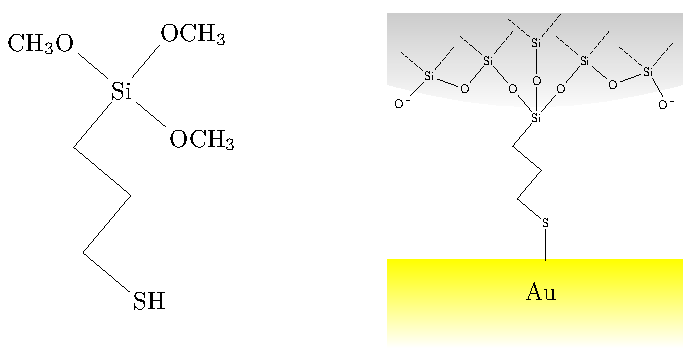
\includegraphics[width=0.60\textwidth]{Esquemas/mod_sup.pdf}
							\caption[Modificación superficial de los electrodos.]{Izquierda: Molécula de  3-mercaptopropil trimetoxisilano\index{mercaptopropil@3-mercaptopropil trimetoxisilano} utilizada como ligante entre los electrodos y las \pdm. Derecha: Esquema pictórico de la modificación superficial con MPTMS.}
							\label{fig:mod_sup}
							\end{center}
							\end{figure}
			
			Una vez realizada la modificación superficial, se llevaron a cabo mediciones EQ, con el objetivo de comparar electrodos modificados y sin modificar, de forma de evaluar el posible bloqueo de los electrodos. La figura \ref{fig:comparaciones_MPTMS} muestra los voltagramas los resultados de dichas comparaciones. Se comparan allí, electrodos con MPTMS y sin MPTMS, recubiertas con \pdm\space y sin recubrir. De estos gráficos comparativos se desprende que el rendimiento electroquímico\index{electroquimico} no se ve afectado significativamente.
	 		
		 			\begin{figure}[th]
			 	   	    \begin{subfigure}[t]{0.49\textwidth}
				        	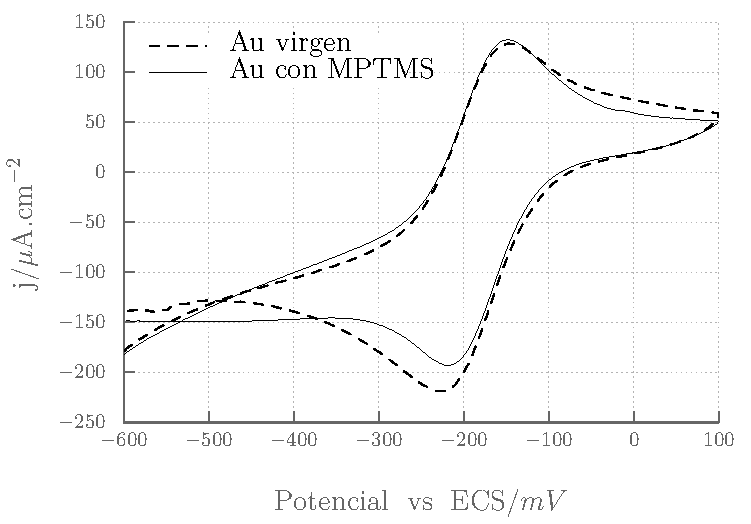
\includegraphics[width=\textwidth]{Graficos/Comparacion_Au-MPTMS.pdf}
				       		\caption{Respuesta EQ de un electrodo desnudo de Au\index{oro} comparado con uno modificado con MPTMS.}	
				       		\end{subfigure}
						\begin{subfigure}[t]{0.49\textwidth}
				 	   	    \includegraphics[width=\textwidth]{Graficos/Comparacion_F127-MPTMS.pdf}
				       		\caption{Respuesta EQ de un electrodo de Au\index{electrodo!de Au}\index{oro} tratados con MPTMS y sin tratar, recubierto con \pdmF\space sobre electrodo de Au\index{electrodo!de Au}.}
				       		\end{subfigure}
						 	\caption[Comparación de superficie\index{superficie}s con y sin MPTMS.]{Voltametrías cíclicas para \aminorutenio\space \SI{1}{\milli\Molar} realizados a \SI{50}{\milli\volt.\second^{-1}} comparando los resultados de electrodos modificados con MPTMS y sin modificar.}
						 \label{fig:comparaciones_MPTMS}	
					     \end{figure}
			
			La segunda estrategía utlizada para promover una mayor adherencia\index{adherencia} de las \pdm\space a los sensores, se basa en minimizar el área de contacto electrodo-mesoporoso. Las mayoría de los resultados discutidos en este capítulo fueron realizados en \pdm\space sobre electrodos plenos de Au. Sin embargo, los sensores\index{sensor} son un conjunto de electrodos o microelectrodo\index{electrodo!microelectrodo}s sobre un sustrato\index{sustrato} dieléctrico (p. ej. SiO$_2$ o vidrio). Eligiendo un diseño adecuado se puede minimizar el área de los electrodos respecto del soporte. De ésta forma las \pdm\space quedan adheridas fuertemente a los sectores donde no está el Au. El resultado final es una película bien adherida sobre una superficie\index{superficie} mixta soporte/electrodos.  La figura \ref{fig:adherencia_microelectrodo} representa de manera esquemática esta situación.
			
				\begin{figure}[!ht]
					\begin{center}
					\includegraphics[width=0.70\textwidth]{Esquemas/adherencia_microelectrodo.pdf}
					\caption[Adherencia a los microelectrodo\index{electrodo!microelectrodo}s.]{Esquema de un corte transversal de los sensores\index{sensor} donde se observan los microelectrodo\index{electrodo!microelectrodo}s y la \pdm\space depositada sobre ellos. Las flechas indican las zonas de baja y alta adherencia.}
					\label{fig:adherencia_microelectrodo}
					\end{center}
					\end{figure}
			
			Ambas estrategias que promueven la adherencia\index{adherencia} de las \pdm\space son complementarias. Esto quiere decir que se puede optimizar el diseño para minimizar la superficie\index{superficie} de electrodos y, a su vez, se pueden tratar los sectores donde queda el Au\index{oro} expuesto con MPTMS, de manera de generar puntos de vinculación entre el mesoporosos y el electrodo. El tratamiento se realiza luego de depositar el Au\index{oro} y antes de realizar el decapado de la fotorresina\index{fotorresina} (consultar sección \ref{sec:fotolito}, pág. \pageref{sec:fotolito}).		
			% Por último decir que se van a usar de ahora en adelante estos sistema, reforzar con bibliografia.

\section{Métodos alternativos de síntesis de \pdm}
	
	 En esta sección se da cuenta de los resultados obtenidos en la fabricación y caracterización de \pdm\space por métodos alternativos a la calcinación\index{calcinación}. Como ya se mencionó anteriormente, el desarrollo de estos métodos surgió de necesidades que emergieron durante el proceso de fabricación de los sensores. Minimizar la diferencia de expansión térmica entre las películas delgadas mesoporosas y metálicas, evitar procesos difusivos, ampliar sustancialmente la gama de sustratos y, mejorar la adherencia\index{adherencia} y disminuir costos, entre otros

	 En este sentido, se idearon procesos que permitan bajar la temperatura (hasta \SI{130}{\celsius}) sin perder grado de condensación\index{condensación} y manteniendo las características espaciales de los poros. Al\index{aluminio} no calcinar, se agrega una etapa extra, la eliminación del surfactante\index{surfactante}. Presentamos a continuación una tabla con la nomenclatura y una breve reseña de los procesos que se exploró.

	 	 \begin{table}[ht!] 
		 	 \caption[Tratamientos alternativos de síntesis de \pdm]{Nomenclatura de los métodos alternativos de síntesis de \pdm.}
			 \begin{tabular}{>{\raggedright\arraybackslash}m{1.9cm}>{\centering\arraybackslash}m{1cm}>{\raggedright\arraybackslash}m{0.9cm}>{\raggedright\arraybackslash}m{6.62cm}} 
			 \toprule
				 Método   &  Nomenclatura$^*$&  & Descripción \\ \midrule
				 Calcinado & CalSC CalSF& &  Condensación\index{condensación} \SI{130}{\celsius} \SI{1}{hora}\hspace{2cm} Extracción \SI{350}{\celsius} \SI{2}{hora}\hspace{2cm} \\ \midrule
				 Simplifciado & SimSC SimSF& &  Condensación\index{condensación} \SI{130}{\celsius} \SI{1}{hora}\hspace{2cm} Extracción IpOH / H$_2$O pH\index{pH}=2 \\ \midrule
				 Prolongado & ProSC ProSF& & Condensación\index{condensación} \SI{130}{\celsius} \SI{7}{dias}\hspace{2cm} Extracción IpOH / H$_2$O pH\index{pH}=2 \\ \midrule				
				 Ácido & ÁciSC ÁciSF& &  Condensación\index{condensación} en atmósfera de HCl\index{acido@ácido!clohídrico}\hspace{2cm} Extracción IpOH / H$_2$O pH\index{pH}=2 \\ \midrule
				 Al\index{aluminio}calino & Al\index{aluminio}cSC Al\index{aluminio}cSF& & Condensación\index{condensación} en atmósfera de NH\index{amoniaco}$_3$\hspace{2cm} Extracción IpOH / H$_2$O pH\index{pH}=2 \\ \midrule
				 Vacío & VacSC VacSF VacZSF& &  Condensación\index{condensación} \SI{130}{\celsius} \SI{7}{dias}, P=\SI{e-5}{\milli\bar}\hspace{2cm} Extracción IpOH / H$_2$O pH\index{pH}=2 \\
				\bottomrule
				   \end{tabular}\vspace*{2pt}
		    	  	\footnotesize{$^*$SC=sílice/CTAB, SF=sílice/F127, ZSF=circonio-sílice/F127}
				   	\label{tabla:tratamientos}
				   \end{table}
				   \vspace*{-0.22cm}

	 Re exponen primero los resultados de las caracterizaciones de las \pdm\space obtenidas por calcinación\index{calcinación}. El propósito de ésto es tener datos de referencia para comparar con los métodos alternativos. Luego, se discuten los resultados que sistemáticamente se obtuvieron por cada uno de ellos. Al\index{aluminio} final de la sección se presenta una tabla (\ref{tabla:resultados}) con todos los resultados obtenidos por cada una de las técnicas, para cada uno de los métodos. Para facilitar la lectura, la mayoría de los gráficos, microscopia\index{microscopía}s y espectros de la sección se encuentran en el anexo C.

	\subsection{Método por calcinación\index{calcinación}}
	 	
	 		El tratamientos por calcinación\index{calcinación} luego del depósito\index{depósito} del sol\index{sol} es una ruta sintética clásica utilizada por muchos autores para la producción de películas delgadas mesoporosas de óxidos\cite{Soler-Illia2002a,Brinker1999,Soler-Illia2006,Grosso2004,Innocenzi2013,anglome2011}. Consiste en estabilizar las \pdm\space en humedad, temperatura y luego calcinar a \SI{350}{\celsius} para calcinar el molde. Los detalles técnicos se pueden consultar en la sección \ref{sec:cond_y_extr}, pág. \pageref{sec:cond_y_extr}.

	 	\subsubsection{Análisis de la porosidad}

		 Como veremos mas adelante la porosidad\index{porosidad} y accesibilidad\index{accesibilidad} nos determinarán la cantidad de analito que se adsorbe o pasa a través de las \pdm, por este motivo es fundamental poder cuantificar dichas características. 

		 Del estudio de las películas por MEB se puede obtener información muy valiosa como tamaño y distribución de los poros\index{distribución!de poro}, así como estudios de la organización espacial de los mismos. En la figura \ref{fig:F127_Si_Au} se muestran imágenes de MEB para películas \pdmF. De éstas, se hace obtiene que se trata de un arreglo de poros con orden local, con tamaños próximos a los de \SI{10}{\nm} de diámetro, coincidiendo la con información existente en la literatura\cite{urade2005,angelome2011,lee2006}.  

			\begin{figure}[th]
		 	   	    \begin{subfigure}[t]{0.49\textwidth}
			        	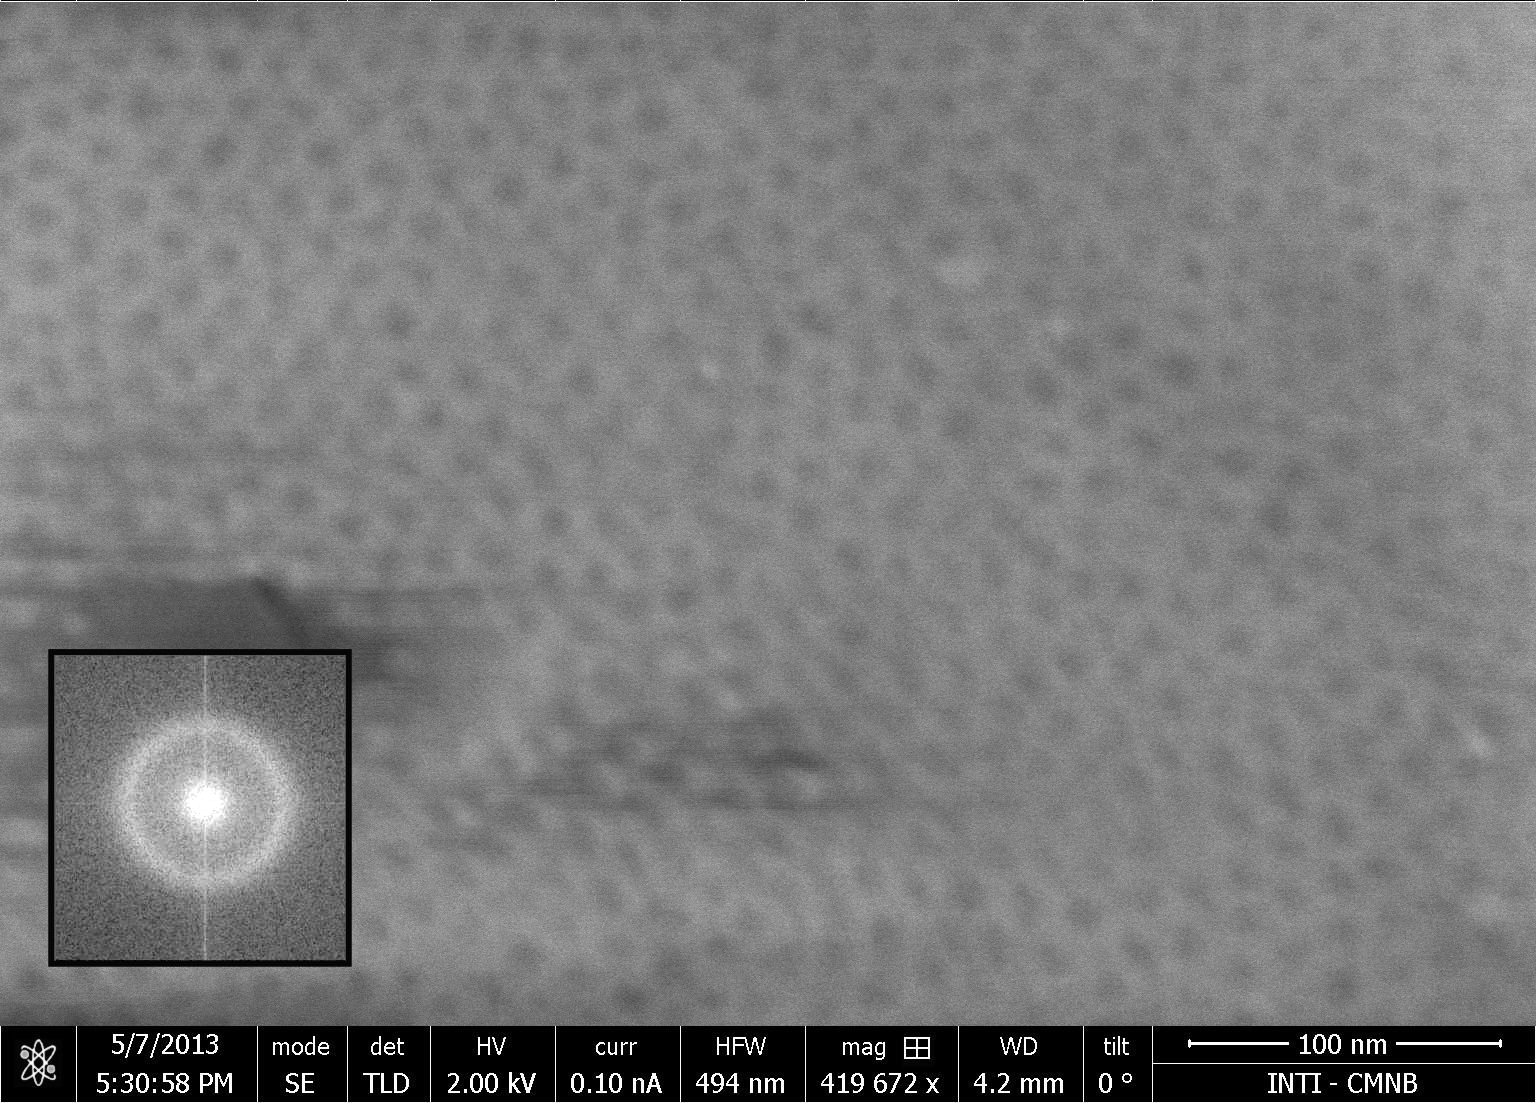
\includegraphics[width=\textwidth]{Imagenes/F127_Si_sup.jpg}
			       		\end{subfigure}
					\begin{subfigure}[t]{0.49\textwidth}
			 	   	    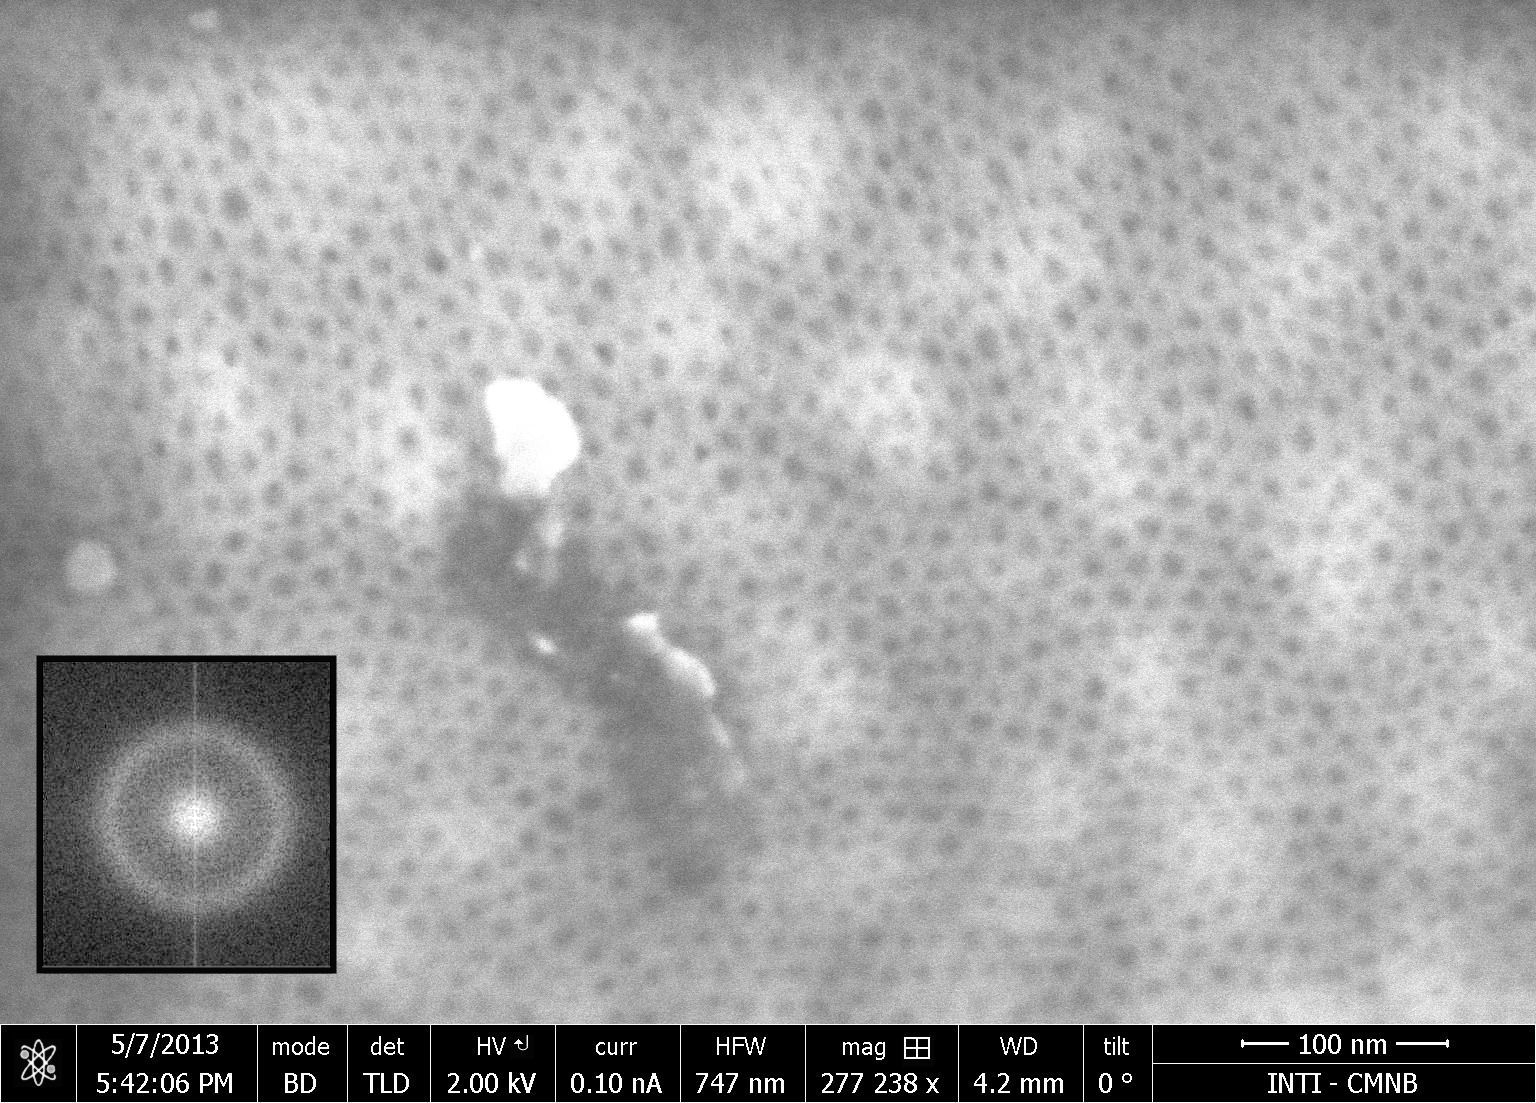
\includegraphics[width=\textwidth]{Imagenes/F127_Au_sup.jpg}
			       		\end{subfigure}
					\caption[MEB arreglo poroso sobre Si y Au.]{Microscopía electrónica de barrido de \pdmF\space donde se observa la distribución y homogeneidad de los poros en superficie\index{superficie}. Izquierda: sobre sustrato\index{sustrato} de silicio. Derecha: sobre sustrato\index{sustrato} de Au.}	 
					 \label{fig:F127_Si_Au}
					 \end{figure}

		 En el caso de las películas porosas estructuras con CTAB es más difícil hacer una análisis por MEB, ya que el diámetro de los poros ($\approx$ \SI{3}{\nm}) esta en el límite de resolución la técnica. Sin embargo, alcanza para  ver que existe un sistema de poros (ver figura \ref{fig:sem_homogeneidad3}). En este caso, para hacer un estudio por imágenes mas completo, se debería recurrir a microscopia\index{microscopía} electrónica de transmisión\index{microscopía!de transmisión} (MET).

		 El estudio por MEB es sumamente útil en muchos aspectos; sin embargo, la información que brinda es de áreas muy pequeñas, superficial y no da información completa sobre la conectividad\index{conectividad} y cuello\index{cuello de poro}s de las películas. Es por ello recurrió a la técnica de elipsoporosimetría\index{elipsoporosimetría ambiental} ambiental (EPA). Es una técnica promedio donde podemos obtener información valiosa sobre la accesibilidad\index{accesibilidad} del agua a los poros, volumen poroso de las \pdm, distribución de tamaños de poros y cuello\index{cuello de poro}s y variación del espesor en función de la presión de vapor\index{presión de vapor} de agua relativa a la presión de saturación ($\text{P/P}_s$). Para valores crecientes de P/P$_s$, la adsorción\index{adsorción} en los mesoporos se produce a través de la formación de una monocapa y luego de multicapas de moléculas de agua sobre las paredes de los poros, seguida de condensación\index{condensación} capilar, es decir, llenado de los poros con agua líquida. La posterior disminución de la presión externa resulta en la desorción\index{desorción} mediante evaporación capilar, vaciando el centro de los poros, seguida por la desorción\index{desorción} de la multicapa de solvente de las paredes de los poros. Para cada punto de P/P$_s$ en equilibrio se tiene un valor del índice de refacción efectivo ($n$), de esta forma se construye la isoterma\index{isoterma} de adsorción\index{adsorción}/desorción de agua. Los cálculos realizados para obtener información estructural (volumen poroso, y distribución de poro\index{poro} y cuello\index{cuello de poro}) a partir de las isoterma\index{isoterma}s se basaron en el protocolo detallado los trabajos del grupo deSánchez\index{Sánchez} y Baklanova\index{Baklanova}\cite{Baklanov2000,Boissiere2005,Sakatani2006}. Los detalles experimentales de esta técnica se presentaron en el capitulo \ref{sec:elipso}, pág. \pageref{sec:elipso}.

		 En las figuras \ref{fig:F127_EPA} y \ref{fig:CTAB_EPA} se presentan las isoterma\index{isoterma}s de adsorción\index{adsorción} de agua para sistemas calcinados \pdmF\space y \pdmC. Se observa que ambas son de tipo IV, según la clasificación de Brunauer\index{Brunauer}\cite{Gregg1967,Violi2015,Fuertes2010}. Este tipo de isoterma\index{isoterma}s con histéresis\index{histéresis} entre la rama de adsorción\index{adsorción} y la de desorción\index{desorción} es característica de materiales con mesoporos, donde los poros se llenan por condensación\index{condensación} capilar. Por otro lado el ciclo de histéresis\index{histéresis} es de tipo H1, según la clasificación IUPAC\index{IUPAC}, lo cual indica poros de tamaño uniforme.\cite{Gregg1967,Lowell2004,Sing1985a}

		 En las figuras \ref{fig:F127_PSD} y \ref{fig:CTAB_PSD} se muestran se muestran las distribuciones de tamaño de poro\index{poro} para estos sistemas. Estas distribuciones se obtuvieron a partir de las isoterma\index{isoterma}s, y se extrajo información estructural tanto de la rama de adsorción\index{adsorción} como de la de desorción\index{desorción}.


		     	  	\begin{figure}[!ht]
		     	  		\begin{subfigure}[t]{0.495\textwidth}
		     	  		\includegraphics[width=\textwidth]{Graficos/SI_F127_Calcinado_EPA.pdf}
						\caption{Elipsoporsimetría de una \pdmF\space depositada sobre silicio\index{silicio} sintetizada por calcinación\index{calcinación}.}
						\label{fig:F127_EPA}
						\end{subfigure}
						\begin{subfigure}[t]{0.495\textwidth}
		     	  		\includegraphics[width=\textwidth]{Graficos/SI_F127_Calcinado_PSD.pdf}
						\caption{Distribución de tamaño de poro\index{poro} y cuello\index{cuello de poro} correspondientes a la isoterma\index{isoterma} de (a).}
						\label{fig:F127_PSD}
						\end{subfigure}
						\caption[Elipsoporosimetría para sistemas \pdmF.]{Curva de adsorción\index{adsorción}/desorción de agua para una \pdmF\space (a). La misma corresponde a una isoterma\index{isoterma} de tipo IV con un lazo de histéresis\index{histéresis} de tipo H1, lo cual se concuerda con materiales mesoporosos con tamaño de poros uniformes. Distribución de poros y cuello\index{cuello de poro}s (b) con tamaño de poros uniformes, de aproximadamente \SI{10}{\nm} de diámetro.}
						\end{figure}
					\begin{figure}[!ht]
		     	  		\begin{subfigure}[t]{0.495\textwidth}
		     	  		\includegraphics[width=\textwidth]{Graficos/SI_CTAB_Calcinado_EPA.pdf}
						\caption{Elipsoporsimetría de una \pdmF\space sobre sustrato\index{sustrato} de silicio\index{silicio} sintetizada por el método clásico de calcinación\index{calcinación}.}
						\label{fig:CTAB_EPA}
						\end{subfigure}
						\begin{subfigure}[t]{0.495\textwidth}
		     	  		\includegraphics[width=\textwidth]{Graficos/SI_CTAB_Calcinado_PSD.pdf}
						\caption{Distribución de tamaño de poro\index{poro} y cuello\index{cuello de poro} correspondientes a la isoterma\index{isoterma} de (a).}
						\label{fig:CTAB_PSD}
						\end{subfigure}
						\caption[Elipsoporosimetría para sistemas \pdmC.]{Curva de adsorción\index{adsorción}/desorción de agua para una \pdmC\space (a). La misma corresponde a una isoterma\index{isoterma} de tipo IV con un lazo de histéresis\index{histéresis} de tipo H1, lo cual se concuerda con materiales mesoporosos con tamaño de poros uniformes. Distribución de poros y cuello\index{cuello de poro}s (b) con tamaño de poros uniformes, de aproximadamente \SI{3}{\nm}.}
						\end{figure}	
		
		 	Del conjunto de resultados presentados se puede resaltar que son películas homogéneas, sin grietas microscopicas, con poroso de orden local y distribución. Las \pdm\space estructuras con F127 presentan poros	y cuello\index{cuello de poro}s de 9 y \SI{4.5}{\nm} de diámetro respectivamente, mientras qeu las estrcuturas con CTAB 2.5 y \SI{2}{\nm}. También se pueden extraer los valores de $n$, porcentaje de volumen poroso (\%V) y espesor los cuales se resumen en la tabla \ref{resultados}. Estos valores son los que se usarán para establecer un parámetros de condensación\index{condensación} y porosidad\index{porosidad} de las \pdm y se usaran como semilla para la discusión comparativa con los resultados obtenidos para el resto de los tratamientos.

	    \subsubsection{Análisis por FTIR}\label{sec:Analisis_IR}

		 Son muchos los trabajos en los cuales caracterizan las películas delgadas de SiO$_2$ por IR\cite{Olsen1989,Almeida1990,Redol1997,Innocenzi2003}, y también muchos que otros que hacen usos de estos resultados \cite{Angelome2008,Calvo2008,Calvo20210}.
		 El análisis de espectroscopia\index{espectroscopia} infrarroja por transformada de Fourier (FTIR) se utilizó en esta tesis para identificar y caracterizar la estructura inorgánica porosa de SiO$_2$, evaluar comparativamente condensación\index{condensación} del óxido, y determinar la presencia de grupos orgánicos, entre ellos residuos de surfactante\index{surfactante}. El seguimiento por FTIR\index{FTIR} de la presencia de surfactante\index{surfactante} es muy importante sobre todo en aquellos tratamientos donde las películas no fueron sometidas a calcinación\index{calcinación}.

		Innocenzi\index{Innocenzi}\cite{Innocenzi2003} ha realizado un análisis completo y bien fundamentado sobre las vibraciones\index{vibración} en el IR, de películas delgadas de SiO$_2$ tanto densas como porososas. Para los enlaces Si-O-Si, se observa la presencia de 4 modos de vibración\index{vibración} óptico-trasversales (TO$_x$) y 4 modos óptico-longitudinales (LO$_x$) para películas delgadas de SiO$_2$. En experimentos de incidencia normal a la superficie\index{superficie}, solo deberían excitarse las vibraciones\index{vibración} óptico-transversales, sin embargo se observan banda de vibraciones\index{vibración} correspondientes a modos óptico-longitudinales asociadas a oscilaciones colectivas acopladas TO-LO.\cite{Pai1986,Grosse1986,Innocenzi2003}.

		 	 \begin{figure}[!ht]
						\begin{center}
						\includegraphics[width=0.85\textwidth]{Graficos/IR_Denso.pdf}
						\caption[FTIR SiO$_2$ denso y SiO$_2$ mesoporoso.]{Espectro de absorción de IR de una película SiO$_2$ denso depositada por \textit{sputtering}\index{sputtering@\textit{sputtering}} comparada con una de SiO$_2$ mesoporoso. Se observa, para las \pdm, la aparición de un marcado hombro en \SI{1180}{\per\cm}debido al acoplamiento TO$_3$-LO$_3$ y un pico correspondiente a la vibración\index{vibración} $\nu$Si-OH.}
						\label{fig:IR-denso}
						\end{center}
						\end{figure}

		 El modo TO$_1$, presenta una banda débil $\approx$\SI{460}{\cm^{-1}} asociada a movimientos de balanceo; el modo TO$_2$ está asociado a un estiramiento simétrico con un pico débil cercano a $\approx$\SI{800}{\cm^{-1}}; y el modo TO$_3$, el cual presenta un pico intenso centrado en $\approx$\SI{1075}{\cm^{-1}}, se encuentra asociado a las vibraciones\index{vibración} asimétricas del enlace Si-O-Si. Respecto de los modos ópticos-longitudinales, LO$_1$ y LO$_2$ no son visibles, y LO$_3$, aparece como un hombro de la banda TO$_3$ a mayores frecuencias. La observación experimental de los modos TO$_4$ y LO$_4$ es escasa, cuando se observa aparecen como bandas débiles en la zona comprendida entre 1200 y \SI{1150}{\cm^{-1}} \cite{Pai1986,Grosse1986}.
				 	
		 Otra observación relevante, realizadas por Al\index{aluminio}meida y Pantano\cite{Almeida1990}, es la naturaleza del hombro presente en $\approx$\SI{1180}{\cm^{-1}}, el cual se intensifica con el aumento de la porosidad\index{porosidad} de la película y lo asocia a un acoplamiento de los modos LO$_3$ y TO$_3$ con predominancia de carácter LO. Este fenómeno parece estar asociado a la dispersión de la radiación\index{radiación} IR dentro de los poros y la consecuente activación del modo longitudinal.	
			
		 Se pudo corroborar dicha observación en los espectros de la figura \ref{fig:IR-denso}, donde se compara una \pdm\space con una película delgada \index{película!delgada}de SiO$_2$ depositada por \textit{sputtering}\index{sputtering@\textit{sputtering}}.  Al\index{aluminio}lí se ve el hombro bien acentuado para la \pdm\space y una banda en $\approx$\SI{965}{\cm^{-1}} asociada al estiramiento Si-OH/Si-O$^-$; mientras que para la película de SiO$_2$ denso se observa la ausencia del hombro, aparición de la incipiente banda de LO$_4$ y desaparece la banda del Si-OH/Si-O$^-$.

		 Además del análisis de la estructura inorgánica, se utilizó FTIR\index{FTIR} para evidenciar la presencia del surfactante\index{surfactante} usado de molde para los poros. Se centrará la atención en las bandas que corresponden a las vibraciones\index{vibración} del enlace C-H, las cuales aparecen en la zona de 2950 a \SI{2850}{\cm^{-1}}. En la figuras \ref{fig:IR_F127_calciando} y \ref{fig:IR_CTAB_calcinado} se comparan \pdm\space calcinadas y sin calcinar para los surfactante\index{surfactante}s utilizados. Se ve como desaparecen las bandas correspondientes a al vibración\index{vibración} C-H debido a la eliminación del surfactate. Se conserva la forma del hombro a $\approx$\SI{1180}{\cm^{-1}} indicador de una estructura porosa y se observa la banda en en $\approx$\SI{965}{\cm^{-1}} asociada al estiramiento Si-OH/Si-O$^-$, el cual según algunos autores sólo desaparece cuando las películas son sometidas a T$>$\SI{500}{\celsius}.\cite{Innocenzi2003,Almeida1990,Bertoluzza1982}

				\begin{figure}[!ht]
						\begin{center}
						\includegraphics[width=0.85\textwidth]{Graficos/IR_F127.pdf}
						\caption[FTIR para una \pdmF.]{Espectro de absorción para una \pdmF\space antes y después de calcinar, donde se puede apreciar la aparición de un pico fuerte el cual correspondiente al surfactante\index{surfactante} F127.}
						\label{fig:IR_F127_calciando}
						\end{center}
						\end{figure}
				
				\begin{figure}[!ht]
						\begin{center}
						\includegraphics[width=0.85\textwidth]{Graficos/IR_CTAB.pdf}
						\caption[FTIR para una \pdmC.]{Espectro de absorción para una \pdmC\space antes y después de calcinar, donde se puede apreciar la aparición de un pico fuerte el cual correspondiente al surfactante\index{surfactante} CTAB.}
						\label{fig:IR_CTAB_calcinado}
						\end{center}
						\end{figure}		
		 
		 Estos espectros IR, obtenidos para películas calcinadas, se utilizaran de parámetro para comparar con los IR de \pdm\space producidas por métodos alternativos. Por un lado, se evalúa la presencia de poros, indicado por la presencia del hombro LO$_3$-TO$_3$. Por otro, el grado de condensación\index{condensación}, siguiendo la relación de picos Si-O-Si/Si-OH. Por último, se corrobora la eliminación del surfactante\index{surfactante} por ausencia de la banda $\approx$\SI{2900}{\per\cm} correspondiente a la vibración\index{vibración} C-H.

		 En la tabla que sigue, se asignan las vibraciones\index{vibración} observadas que servirán de referencia para el análisis de resultados de las próximas seccciones.

		 	\begin{table}[ht!] 
		 	 \caption[Asignación de vibraciones\index{vibración} en el IR]{Bandas y asignación de vibraciones\index{vibración} en el IR frecuentemente observadas a lo largo de la tesis.}
			 \begin{tabular}{>{\raggedright\arraybackslash}m{2.6cm}>{\centering\arraybackslash}m{2.55cm}>{\raggedright\arraybackslash}m{5.7cm}} 
			 \toprule
				 Posición (\si{\per\cm})   &  Vibración &  Presente en \\ \midrule
				 3500-3000	& $\nu_\text{OH}$ & H$_2$O, 2-propanol\index{propanol@2-propanol} \\ \midrule
				 2950-2850  & $\nu_\text{C-H}$ & Molde (CTAB, Pluronic F127\index{Pluronic F127}) \\ \midrule
				 2450		& CO$_2$ & CO$_2$ ambiental \\ \midrule
				 2000-1200  & H$_2$O & Estructura fina del H$_2$O \\ \midrule
				 1250		& $\nu_\text{Si-O-Si}$ & SiO$_2$ Denso LO$_3$ \\ \midrule
				 1170		& $\nu_\text{Si-O-Si}$ & SiO$_2$ Denso LO$_4$ \\ \midrule
				 1075		& $\nu_\text{Si-O-Si}$ & SiO$_2$ TO$_3$ \\ \midrule
				 1180 (hombro) & $\nu_\text{Si-O-Si}$ & SiO$_2$ poroso acoplamieno LO$_3$-TO$_3$ \\ \midrule
				 965 		& $\nu_\text{Si-OH}$ & SiO$_2$ parcialmente condensado\\ \midrule 
				 800		& $\nu_\text{Si-O-Si}$ & SiO$_2$ TO$_2$ \\
				 \bottomrule
				   \end{tabular}
				   	\label{tabla:ftir}
				   \end{table}

	    \subsubsection{Accesibilidad de las PDM}

			Hasta ahora se han evaluado muchos de los aspectos fundamentales para poder pensar en utilizar las películas mesoporosas de óxido de silicio\index{silicio!oxido de}\index{silicio} como componentes de sensores: estructura porosa, volumen poroso, compatibilidad de sustratos, técnicas de depósito, control del espesor, etc. 

			Sin embargo, se debe tener en cuenta un aspecto crítico para utilizar estas películas como parte de un sensor\index{sensor} electroquímico\index{electroquimico}. Se tiene que garantizar el libre acceso de los analitos a través de los nanoporos, de forma de poder difundir hasta la superficie\index{superficie} del electrodo, y que tenga lugar allí, la reacción electroquímica\index{electroquimico}.

			Para ello, se coloca una solución con una sonda\index{sonda} electroquímica\index{electroquimico} adecuada, en la celda de medición. La forma en que fueron tomadas las medidas se explica en la sección \ref{sec:medidas_eq}, pág \ref{sec:medidas_eq}. 

			La figura \ref{fig:accesibilidad} muestra dos voltametrías cíclicas, una para \pdmF\space y otra para \pdmC en presencia de \aminorutenio\space \SI{1}{\milli\Molar} en solución de KCl \SI{0.1}{\Molar}. En ambos voltagramas se registra una respuesta electroquímica\index{electroquimico}, demostrando que la superficie\index{superficie} del electrodo se encuentra accesible. Los resultados sugieren que existe un camino percolativo en las \pdm, tanto si se estructuran con F127 o con CTAB, que permite, o bien que la señal electroquímica\index{electroquimico} se propague desde el seno de la solución hasta el electrodo o bien que el analito difunda desde la solución al electrodo. Los fenómenos de trasporte involucrados en este experimento, son tema central de esta tesis y se discuten en detalle en el capitulo \ref{chap:Electroquimica}, así como la forma de los voltagramas. En dicho capítulo se analizan la separación del potencial entre los picos anódico y catódico y las intensidades de los mismos relativa a un electrodo de Au\index{electrodo!de Au}\index{oro} sin recubrir. 

						\begin{figure}[th]
				 	   	    \begin{subfigure}[t]{0.495\textwidth}
				        	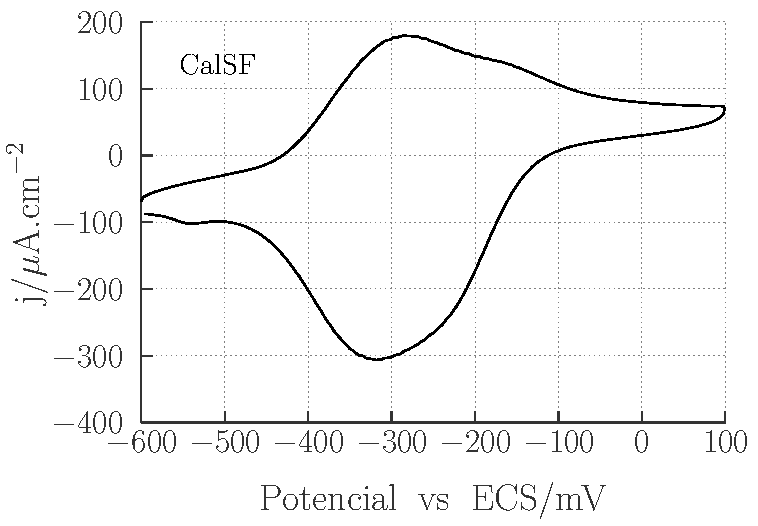
\includegraphics[width=\textwidth]{Graficos/SF-accesibilidad.pdf}
				       		\caption{Voltametría Cíclica sobre \pdmF}
				         	\end{subfigure}
				         	\begin{subfigure}[t]{0.495\textwidth}
				        	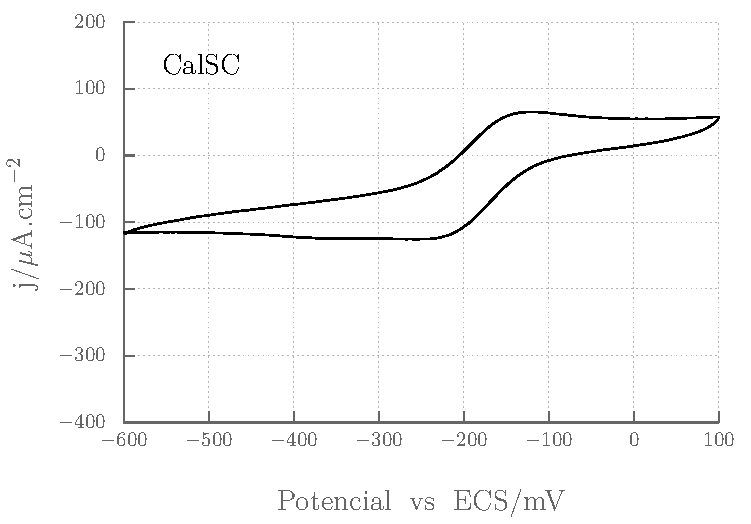
\includegraphics[width=\textwidth]{Graficos/SC-accesibilidad.pdf}
				       		\caption{Voltametría Cíclica sobre \pdmC}
				         	\end{subfigure}
				     		\caption[Accesibilidad electrodo de trabajo\index{electrodo!de trabajo}.]{Voltametrías Cíclicas de \aminorutenio\space \SI{1}{\milli\Molar} sobre Au\index{oro} recubierto con \pdm con una velocidad de barrido\index{velocidad!de barrido} \SI{50}{\milli\volt\per\second} usando de referencia ESC.}
				     		\label{fig:accesibilidad}
				     		\end{figure}

			%El fenomeno de transporte\index{transporte} de sonda\index{sonda}s electroquimicas a través de las \pdm\space es un tema cemtral de este trabajo y se trata en profundidad en el capitulo.... por ahora 
			%Por tecnicas de VC. Distinguir entre accesibilidad\index{accesibilidad} de los poros y accesibilidad\index{accesibilidad} para llegar al electrodo y un camino de percolación para llegar al fondo.
	
	 \subsection{Método simplificado}

	 	De todos los tratamientos pos-depósito, es el mas simple de todos. Consistió en estabilizar la \pdm a \SI{130}{\celsius} durante \SI{1}{\hour} y luego extraer el surfactante\index{surfactante} en un reflujo de 2-pronanol durante \SI{15}{\minute}. 
		
		En el análisis por microscopia\index{microscopía} se aprecia que las \pdmF\space sometidas a éste tratamiento se adhieren bien y quedan bien formadas, sin grietas ni discontinuidades y con poros bien formados sobre la superficie\index{superficie} para ambos sustratos, tanto sobre Au\index{oro} como sobre Si \ref{fig:Microscopia_F127_simplificado}. Las \pdmC\space sobre silicio\index{silicio} también adhieren bien y no presentan grietas. Sobre Au\index{oro} las \pdm\space presentan grietas y discontinuidades en su estructura (figura \ref{fig:Microscopia_CTAB_simplificado}), lo cual se adjudica al hecho de la adsorción\index{adsorción} del bromuro sobre el Au, tema que ya fue discutido en la sección \ref{sec:adherencia}, pág. \pageref{sec:adherencia}. 
		
		La caracterización por elipsoporismetría para las \pdmF\space resulto en una isoterma\index{isoterma} tipo IV con histéresis\index{histéresis} HX para las \pdmC y tipo IV con histéresis\index{histéresis} HX para las \pdmF.\cite{}. Los sitemas estructurados con CTAB presentan una porosidad\index{porosidad} es alta, aproximadamente 40\%, sin embargo la isoterma\index{isoterma} muestra una histésis pequeña entre las ramas de adsorción\index{adsorción} y desorción\index{desorción}. Esto significa, que no hay prácticamente diferencia entre el tamaño de poro\index{poro} y cuello\index{cuello de poro} (figuras \ref{fig:CTAB_simplificado_EPA}  y \ref{fig:CTAB_simplificado_PSD}). Este diámetro de poro\index{poro} pequeño se puede atribuir a que el surfactante\index{surfactante} ha sido sólo parcialmente eliminado de la estructura, estrechando el tamaño de poro\index{poro} hasta hacerlo prácticamente igual tamaño de los cuello\index{cuello de poro}s.
		En el caso de los sistemas \pdmF\space la adsorcion de agua se produce en una única etapa mientras que la desorción\index{desorción} ocurren en dos a P/P$_s=0,65$ y  P/P$_s=0,45$ (figura \ref{fig:F127_simplificado_EPA}). Thielemann\index{Thielemann} \cite{Thielemann2011} y Groen\index{Groen}\cite{Groen2003} proponen que este comportamiento, se produce al desorber el agua ocluida en poros que están más o menos <<bloqueados>> por el diámetro de los cuello\index{cuello de poro}s. Al\index{aluminio} producirse la desorción\index{desorción} del agua a través de cuello\index{cuello de poro}s de distinto tamaño, la fuerza  necesaria para vencer la tensión superficial\index{tensión superficial} debe ser mayor, desorbiendo a menores P/P$s$ cuanto menores sea el diámetro de los cuello\index{cuello de poro}s; tal como predice la ecuación de Kelvin\index{Kelvin} (ver ecuación {\ref{eq:kelvin}). Esta observación se repite para varios de los tratamientos, 



		en el IR (figura \ref{fig:IR_CTAB_simplificado}) se ve dicho residuo en el espectro correspondiente a la película extraída con 2-pronanol. El hecho de exista esa cantidad de residuo remanente, se lo atribuye a la baja condensación\index{condensación} que presentan las películas con este tratamiento, ya que de queda surfactante\index{surfactante} retenido en la red de silice\index{silicio!oxido de} parcialmente condensada.


		En la figuras \ref{fig:IR_F127_simplificado} se comparan el espectro de absorción en el IR para una \pdmF\space antes y después de practicar la extracción\index{extracción} del surfactante\index{surfactante}. Se ve como desaparece el pico correspondiente al surfactante\index{surfactante} (estiramiento C-H) luego de la extracción\index{extracción}. También se observa la típica banda de la vibración\index{vibración} TO$_3$ de silice\index{silicio!oxido de} mesoporosa\index{película!mesoporosa} en $\approx \text{\SI{1070}{\cm^{-1}}}$.

	 \subsection{Método prolongado}

	 \subsection{Método ácido}

	 \subsection{Método alcalino}

	 \subsection{Método por alto vacio\index{alto@alto vacío}}

	 \subsection{Comparación de resultados}

	 	% \begin{table}[ht!] 
		 % 	 \caption[Compación de resultados \pdm]{asdasdasdasd \pdm.}
			%  \begin{tabular}{>{\raggedright\arraybackslash}m{1.9cm}>{\centering\arraybackslash}m{1cm}>{\raggedright\arraybackslash}m{0.9cm}>{\raggedright\arraybackslash}m{6.62cm}} 
			%  \toprule
			% 	 Método   &  Nomenclatura$^*$&  & Descripción \\ \midrule
			% 	  CalC    & 				&   &  			\\ \midrule	
			% 	  CalSF   & 				&   &  			\\
			% 	\bottomrule
			% 	   \end{tabular}\vspace*{2pt}
		 %    	  	\footnotesize{$^*$SC=sílice/CTAB, SF=sílice/F127, ZSF=circonio-sílice/F127}
			% 	   	\label{tabla:tratamientos}
			% 	   \end{table}

		\begin{table}[ht!] 
		 	 \caption[Compación de resultados \pdm]{asdasdasdasd \pdm.}
			 \begin{tabular}{>{\raggedright\arraybackslash}m{1.5cm}|>{\centering\arraybackslash}m{1cm}>{\centering\arraybackslash}m{1cm}>{\centering\arraybackslash}m{1cm}>{\centering\arraybackslash}m{1cm}>{\centering\arraybackslash}m{1cm}>{\centering\arraybackslash}m{1cm}>{\centering\arraybackslash}m{1cm}} 
			 \toprule
				 \multirow{2}{*}{Método}& \multicolumn{2}{c}{Microscopia$^*$} & \multicolumn{5}{c}{Elipsoporosimetría$*$} \\
    			   		 & Si & Au\index{oro} & dp & dc & P & esp & n \\ \midrule
    			 CalSC   & B  & m  & 5  & 2  & 40\% & 220 & 1.25 \\ 
  	 	         CalSF   & B  & m  & 5  & 2  & 40\% & 220 & 1.25 \\ \midrule
  	 	         SimSC   & B  & m  & 5  & 2  & 40\% & 220 & 1.25 \\ 
			     SimSF   & B  & m  & 5  & 2  & 40\% & 220 & 1.25 \\  
		 %\multirow{2}{*}{Métodos}   & Microscopia  \\  \midrule
		 %FALTA ANGULO DE CONTACTO!!!!
				 % CalC   					&  \multicolumn{2}{c}&X	\\ \midrule	
				 % CalSF   					&    			\\
				\bottomrule
			\end{tabular}\vspace*{2pt}
		    \footnotesize{$^*$se evalúa la adherencia, presencia de grietas o discontinuidades y la apariencia superficial de los poros.}
			\label{tabla:resultados}
			\end{table}
		
		\begin{table}[ht!] 
		 	 \caption[Compación de resultados \pdm]{asdasdasdasd \pdm.}
			 \begin{tabular}{>{\raggedright\arraybackslash}m{1.5cm}|>{\centering\arraybackslash}m{1cm}>{\centering\arraybackslash}m{1cm}>{\centering\arraybackslash}m{1cm}>{\centering\arraybackslash}m{1cm}>{\centering\arraybackslash}m{1cm}>{\centering\arraybackslash}m{1cm}>{\centering\arraybackslash}m{1cm}} 
			 \toprule
				 \multirow{2}{*}{Método}& \multicolumn{2}{c}{FTIR$^*$} & \multicolumn{2}{c}{EQ accesibilida$*$} & Observaciones \\
    			   		 & cond & extra & EQ & dc & P & esp & n \\ \midrule
    			 CalSC   & B  & m  & 5  & 2  & 40\% & 220 & 1.25 \\ 
  	 	         CalSF   & B  & m  & 5  & 2  & 40\% & 220 & 1.25 \\ \midrule
  	 	         SimSC   & B  & m  & 5  & 2  & 40\% & 220 & 1.25 \\ 
			     SimSF   & B  & m  & 5  & 2  & 40\% & 220 & 1.25 \\  
		 %\multirow{2}{*}{Métodos}   & Microscopia  \\  \midrule
				 % CalC   					&  \multicolumn{2}{c}&X	\\ \midrule	
				 % CalSF   					&    			\\
				\bottomrule
			\end{tabular}\vspace*{2pt}
		    \footnotesize{$^*$se evalúa la adherencia, presencia de grietas o discontinuidades y la apariencia superficial de los poros.}
			\label{tabla:resultados}
			\end{table}					 	  
				   
\section{Discusión sobre los métodos}

	\subsection{Sobre los sustratos}

	\subsection{Sobre la condensación\index{condensación}}

	\subsection{Sobre el surfactante\index{surfactante}}

	\subsection{Sobre la respuesta electroquímica\index{electroquimico}}

\section{Conclusiones parciales}

	En este capitulo se presentan los primeros resultados que se obtuvieron en el proceso de fabricación, desarrollo y caracterización de los sensores\index{sensor} electroquímico\index{electroquimico}s\index{electroquimico} permeoselectivos basados en películas delgadas de óxido de silicio\index{silicio!oxido de}. Se lograron sintetizar las películas mesoporosas de óxido de silicio\index{silicio!oxido de}\index{silicio} sobre diferentes sustratos, silicio, vidrio, oro\index{oro} y microelectrodo\index{electrodo!microelectrodo}s. Se utilizaron dos agentes moldeantes F127 y CTAB y seguió la vía clásica de calcinación\index{calcinación} a \SI{350}{\celsius} para condensación\index{condensación} del SiO$_2$ y calcinación\index{calcinación} del surfactante\index{surfactante}. Teniendo en cuenta las herramientas y procesos propios de la microelectronica, para el deposito del sol, se eligió usar exclusivamente el método de \textit{spin-coating}\index{spin@\textit{spin-coating}}. Se regulo el espesor de las películas al deseado, entre 200 y \SI{250}{\nm} para que no se produzcan fracturas y discotinuidades en las películas. Frente a los problemas encontrados de adherencia\index{adherencia} a los electrodos de Au\index{electrodo!de Au} se utilizaron dos estrategias: modificación química y optimización del diseño de los electrodos. Mejorada la adherencia\index{adherencia} se demostró que el desempeño electroquímico\index{electroquimico} no se vio afectado. 

	Las películas fueron caracterizadas por microscopia\index{microscopía} electrónica\index{microscopía!electrónica}, elipsoporossimetría, espectroscopia\index{espectroscopia} IR y electroquimicamente. De estas caracterización se demostró que las películas son homogéneas en espesor, en superficie\index{superficie}, de poroso uniformes en tamaño y distribución y que existe un camino percolativo del seno de la solución a la superficie\index{superficie} del electrodo, permitiendo realizar reacciones de óxido/reducción sobre la superficie\index{superficie} del electrodo.

%destacados:

%Agregar mas adelante que se puede utilizar para sistemas mas adelante como bicapa sobre F127, demostrado en otros paper bla bla y poner bibliografía. Anduvo en parte para el calcinado.

%Siempre con la idea de desarrollar un multisensor electroquímico\index{electroquimico}s\index{electroquimico} selectivo, especifico, integrado y escalable decidimos, para logra este fin, explorar las propiedades de las películas delgadas de óxidos mesoporosos descritas con anterioridad. Nos dedicamos, como primera aproximación, a depositar estas películas de óxido sobre otra película delgada, esta vez de Au, que a su vez está depositada sobre algún sustrato\index{sustrato} rígido y térmicamente estable como vidrio\index{vidrio} u silicio, de forma de obtener una estructura bicapa electrodo$|$mesoporoso. 

	%Muchos de los trabajos que figuran el la bibliografía utilizan técnicas de electroquímica\index{electroquimico} como herramienta de caracterización para películas mesoporosas con múltiples propósitos; como inferir estructuras de poros, accesibilidad, deducir propiedades de transporte\index{transporte} y estimar variables del sistema. En este trabajo se plantea el uso de la electroquímica\index{electroquimico}, no solo como herramienta de caracterización de películas mesoporososas sino también como técnica analítica. Para lograr dicho objetivo se evaluó el desempeño electroquímico\index{electroquimico} de los electrodos de Au\index{electrodo!de Au} así como la viabilidad de ser utilizados como sustrato\index{sustrato} para el depósito\index{depósito} de película delgada \index{película!delgada}mesoporosa. Dichas películas serán el elemento activo, que actúa como membrana selectiva de los analitos electroactivos a cuantificar. 


%Control de espesor
%Tecnicas compatible spin-coating
%Sobre Au\index{oro} - todo bien! sobre si / vidrio
% sistemas porosos, accesibles, homogeneos con llegada al electrodo.
% Problemas de adhesion y soolucion con molecula de MPTMS
% Limitaciones!!! Calcinacion....


